\title{Video compression fundamentals}
\author{Vicente González Ruiz}
\maketitle
\tableofcontents

\section{\mylink{redundancy}{Sources of redundancy}}

\section{Block-based MC (Motion Compensation)~\cite{rao1996techniques}}
\begin{itemize}
\tightlist
\item
  Usually, only performed by the encoder (compress one. decompress
  many).
\item
  MC removes temporal redundancy. A \emph{predicted image} can be
  encoded as the difference between it and another image called
  \emph{prediction image} which is a motion compensated projection of
  one or more images named \emph{reference images}. ME tries to
  generate \emph{residue images} as close as possible to the null
  images.
\item
  For example, in the MPEG-1 standard, the reference image/s is/are
  divided in blocks of $16\times 16$ pixels called \emph{macroblocks}.
\item
  Each reference block is searched in the predicted image and the best
  match is indicated by mean of a \emph{motion vector}.
\item
  Depending on the success of the search and the number of reference
  images, the macroblocks are classified into:

  \begin{itemize}
  \tightlist
  \item
    \textbf{I (intra)}: When the compression of residue block generates
    more bits than the original (predicted) one.
  \item
    \textbf{P (predicted)}: When it is better to compress the residue
    block and there is only one reference macroblock.
  \item
    \textbf{B (bidirectionally predicted)}: The same, but if we have two
    reference macroblocks.
  \item
    \textbf{S (skipped)}: When the energy of the residue block is
    smaller than a given threshold.
  \end{itemize}
\item
  I-pictures are composed of I macroblocks, only.
\item
  P-pictures do not have B macrobocks.
\item
  B-pictures can have any type of macroblocks.
\end{itemize}

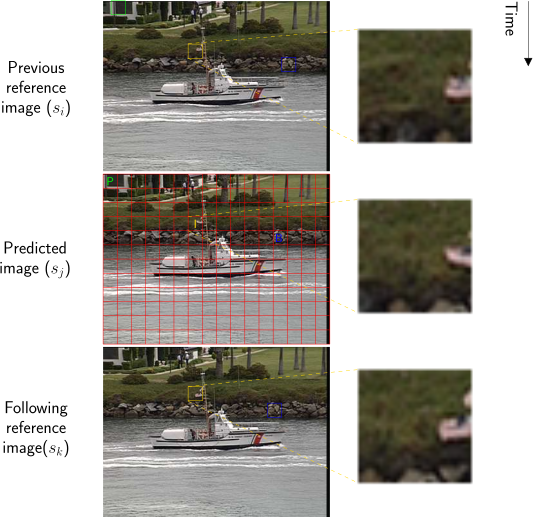
\includegraphics{macroblocks}

\section{Sub-pixel accuracy}

\begin{itemize}
\tightlist
\item
  The motion estimation can be carried out using integer pixel accuracy
  or a fractional (sub-) pixel accuracy.
\item
  For example, in MPEG-1, the motion estimation can have up to 1/2 pixel
  accuracy. A bi-linear interpolator is used:
\end{itemize}
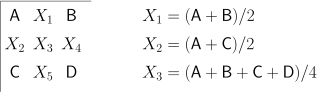
\includegraphics{interpolation}

\section{Matching criteria (similitude between macroblocks)}
\begin{itemize}
\item
  Let $a$ and $b$ the macroblocks which we want to compare. Two main
  distortion metrics are commonly used:

  \begin{itemize}
  \item
    \textbf{MSE (Mean Square Error)}:

    \begin{equation}
      \frac{1}{16\times 16}\sum_{i=1}^{16}\sum_{j=1}^{16}(a_{ij}-b_{ij})^2
    \end{equation}
  \item
    \textbf{MAE (Mean Absolute Error)}:

    \begin{equation}
      \frac{1}{16\times 16}\sum_{i=1}^{16}\sum_{j=1}^{16}|a_{ij}-b_{ij}|
    \end{equation}
  \end{itemize}
\item
  These similitude measures are used only by MPEG compressors.
  Therefore, any other one with similar effects (such as the error
  variance or the error entropy) could be used also.
\item
  Other less common distortion metrics that can work are:

  \begin{itemize}
  \item
    \textbf{EE (Error
    \href{https://en.wikipedia.org/wiki/Entropy_(information_theory)}{Entropy}}:

    \begin{equation}
      -\frac{1}{16\times 16}\sum_{i=1}^{16}\sum_{j=1}^{16}\log_2(a_{ij}-b_{ij})p(a_{ij}-b_{ij})
    \end{equation}
  \end{itemize}
\end{itemize}

\section{Searching strategies}
\begin{itemize}
\item
  Only performed by the compressor.

  \begin{itemize}
  \tightlist
  \item
    \textbf{Full search}: All the possibilities are checked. Advantage:
    the best compression. Disadvantage: CPU killer.
  \end{itemize}

  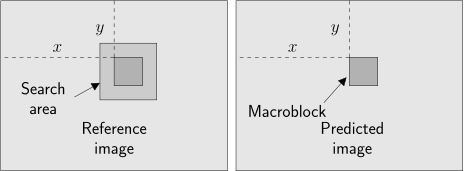
\includegraphics{full_search}
  
  \begin{itemize}
  \tightlist
  \item
    ** Logaritmic search**: It is a version of the full search algorithm
    where the macro-blocks and the search area are sub-sampled. After
    finding the best coincidence, the resolution is increased in a power
    of 2 and the previous match is refined in a search area of
    $\pm 1$, until the maximal resolution (even using subpixel
    accuracy) is reached.
  \end{itemize}

  \begin{itemize}
  \tightlist
  \item
    \textbf{Telescopic search}: Any of the previously described
    techniques can be speeded up if the searching area is reduced. This
    can be done supposing that the motion vector of the same macro-block
    in two consecutive images is similar.
  \end{itemize}
\end{itemize}

\section{The GOP (Group Of Pictures) concept}
\begin{itemize}
\tightlist
\item
  The temporal redundancy is exploited by blocks of images called GOPs.
  This means that a GOP can be decoded independently of the rest of
  GOPs. Here an example:
\end{itemize}

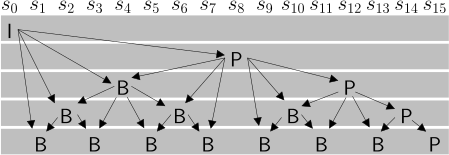
\includegraphics{GOPs}

\section{MCTF (Motion Compensated Temporal Filtering)}
\begin{itemize}
\tightlist
\item
  This is a DWT where the input samples are the original video images
  and the output is a sequence of residue images.
\end{itemize}

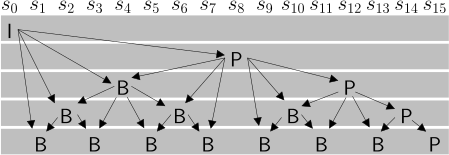
\includegraphics{GOPs}%{6cm}{600}

\section{$\pm$ 1-spiral-search ME (Motion Estimation)}
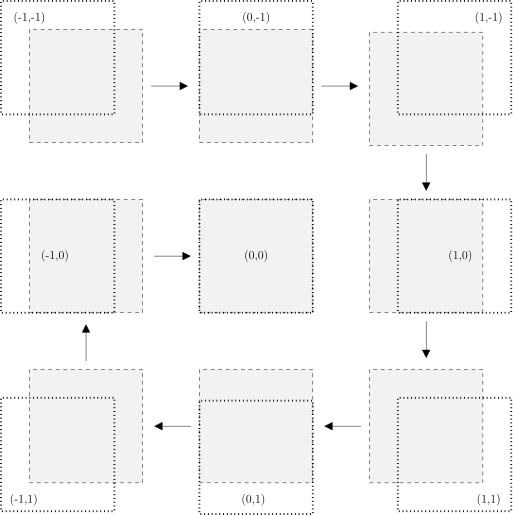
\includegraphics{spiral_search}%{6cm}{600}

\section{Linear frame interpolation using block-based motion compensation}
\label{sec:linear_frame_interpolation}
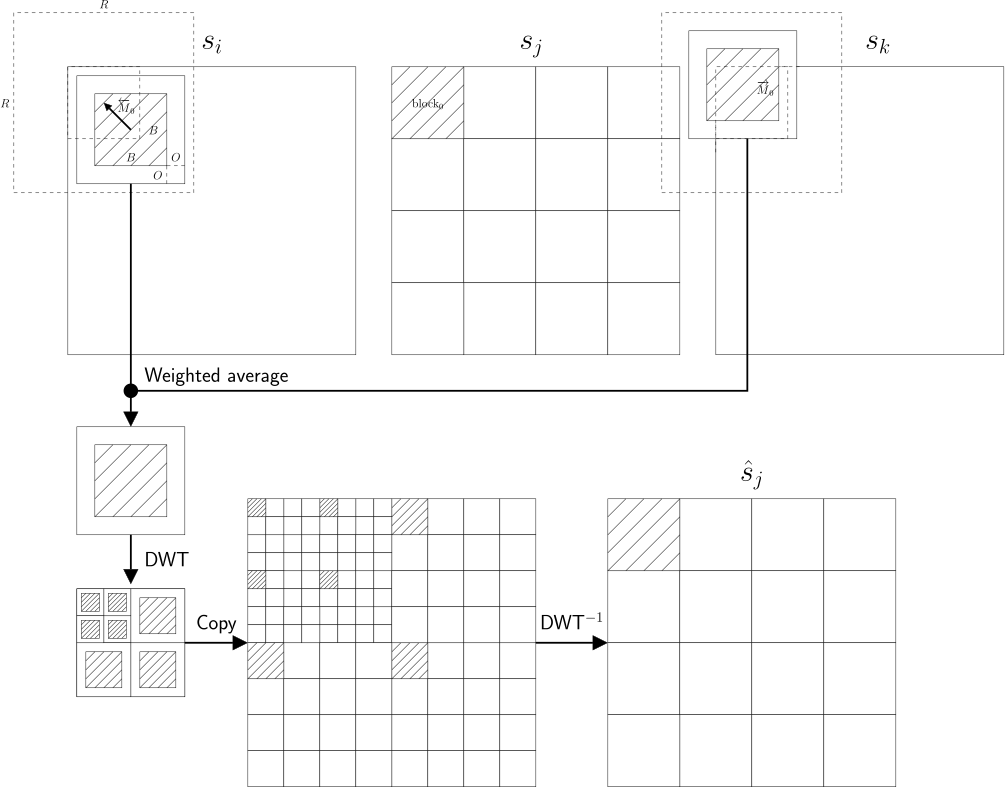
\includegraphics{frame_interpolation}%{10cm}{1000}

\subsection{Input}
\begin{itemize}
\tightlist
\item
  $R$: square search area, in pixels.
\item
  $B$: square block size, in pixels.
\item
  $O$: border size, in pixels.
\item
  $s_i$, $s_j$ and $s_k$ three chronologically ordered,
  equidistant frames, with resolution $X\times Y$.
\item
  $A$: $\frac{1}{2^A}$ subpixel accuracy.
\end{itemize}

\subsection{Output}
\begin{itemize}
\tightlist
\item
  $\hat{s}_j$: a prediction for frame $s_j$.
\item
  $m$: a matrix with $\lceil X/B\rceil \times \lceil Y/B\rceil$
  bidirectional motion vectors.
\item
  $e$: a matrix with $\lceil X/B\rceil \times \lceil Y/B\rceil$
  bidirectional Root Mean Square matching Wrrors (RMSE).
\end{itemize}

\subsection{Algorithm}
\begin{enumerate}
\tightlist

\item
  Compute the DWT$^l$, where $l=\lfloor\log_2(R)\rfloor-1$ levels,
  of the predicted frame $s_j$ and the two reference frames $s_i$
  and $s_k$.
  \href{https://vicente-gonzalez-ruiz.github.io/video_compression/graphics/frame_interpolation_step_1.svg}{Example}.

\item
  $LL^l(m)\leftarrow 0$, or any other precomputed values (for example,
  from a previous ME in neighbor frames).
  \href{https://vicente-gonzalez-ruiz.github.io/video_compression/graphics/frame_interpolation_step_2.svg}{Example}.

\item
  Divide the subband $LL^l(s_j)$ into blocks of size $B\times B$
  pixels, and $\pm 1$-spiral-search them in the subbands $LL^l(s_i)$
  and $LL^l(s_k)$, calculating a low-resolution
  $LL^l(m)=\{LL^l(\overleftarrow{m}), LL^l(\overrightarrow{m})\}$
  bi-directional motion vector field. 
  \href{https://vicente-gonzalez-ruiz.github.io/video_compression/graphics/frame_interpolation_step_3A.svg}{Example}.
  \href{https://vicente-gonzalez-ruiz.github.io/video_compression/graphics/frame_interpolation_step_3A_bis.svg}{Example}.
\item
  While $l>0$:
  
  \begin{enumerate}
    
  \item
    Synthesize $LL^{l-1}(m)$, $LL^{l-1}(s_j)$, $LL^{l-1}(s_i)$
    and $LL^{l-1}(s_k)$, by computing the 1-level DWT$^{-1}$.
    \href{https://vicente-gonzalez-ruiz.github.io/video_compression/graphics/frame_interpolation_step_4A.svg}{Example}.
    \href{https://vicente-gonzalez-ruiz.github.io/video_compression/graphics/frame_interpolation_step_4A_bis.svg}{Example}

  \item
    $LL^{l-1}(M)\leftarrow LL^{l-1}(M)\times 2$.
    \href{https://vicente-gonzalez-ruiz.github.io/video_compression/graphics/frame_interpolation_step_4B.svg}{Example}.
  
  \item
    Refine $LL^{l-1}(m)$ using $\pm 1$-spiral-search.
    \href{https://vicente-gonzalez-ruiz.github.io/video_compression/graphics/frame_interpolation_step_4C.svg}{Example}.
  
  \item
  $l\leftarrow l-1$. (When $l=0$, the motion vectors field $m$
  has the structure:)
  
  \end{enumerate}
  
  \href{https://vicente-gonzalez-ruiz.github.io/video_compression/graphics/motion_vectors.svg}{Example}.
  
\item
  While $l<A$ (in the first iteration, $l=0$, and $LL^0(M):=M$):
  
  \begin{enumerate}
  \item
    $l\leftarrow l+1$.
    
  \item
    Synthesize $LL^{-l}(s_j)$, $LL^{-l}(s_i)$ and $LL^{-l}(s_k)$,
    computing the 1-level DWT$^{-1}$ (high-frequency subbands are
    $0$). This performs a zoom-in in these frames using $1/2$-subpixel
    accuracy. 
    
    \href{https://vicente-gonzalez-ruiz.github.io/video_compression/graphics/frame_interpolation_step_5B.svg}{Example}.
    
  \item
    $m\leftarrow m\times 2$.
    
    \href{https://vicente-gonzalez-ruiz.github.io/video_compression/graphics/motion_vectors_by_2.svg}{Example}.
    
  \item
    $B\leftarrow B\times 2$.
    
  \item
    Divide the subband $LL^{-l}(s_j)$ into blocks of $B\times B$
    pixels and $\pm 1$-spiral-search them into the subbands
    $LL^{-l}(s_i)$ and $LL^{-l}(s_k)$, calculating a $1/2^l$
    sub-pixel accuracy $m$ bi-directional motion vector field. 
    \href{https://vicente-gonzalez-ruiz.github.io/video_compression/graphics/motion_vectors_definitive.svg}{Example}.
    
  \item
    Frame prediction. For each block $b$:
    
  \item
    Compute
    \begin{equation}
      \hat{b}\leftarrow \frac{b_i\big(\overleftarrow{e}_{\text{max}}-\overleftarrow{e}(b)\big) + b_k\big(\overrightarrow{e}_{\text{max}}-\overrightarrow{e}(b)\big)}{\big(\overleftarrow{e}_{\text{max}}-\overleftarrow{e}(b)\big) + \big(\overrightarrow{e}_{\text{max}}-\overrightarrow{e}(b)\big)},
    \end{equation}
    
    where $\overleftarrow{e}(b)$ is the (minimum) distortion of the
    best backward matching for block $b$, $\overrightarrow{e}(b)$
    the (minimum) distortion of the best forward matching for block
    $b$,
    $\overleftarrow{e}_{\text{max}}=\overrightarrow{e}_{\text{max}}$ are
    the backward and forward maximum matching distortions, $b_i$ is
    the (backward) block found (as the most similar to $b$) in frame
    $s_i$ and $b_k$ is the (forward) block found in frame
    $s_k$. Notice that, if
    $\overleftarrow{e}(b)=\overrightarrow{e}(b)$, then the
    prediction is
    \begin{equation}
      \hat{b} = \frac{b_i + b_k}{2},
    \end{equation}
    and if $\overleftarrow{e}(b)=0$,
    \begin{equation}
      \hat{b} = b_k,
    \end{equation} and viceversa.
  \end{enumerate}
\end{enumerate}

\subsection{Lab}
Implement the Section \ref{sec:linear_frame_interpolation} (work on
\url{https://github.com/Sistemas-Multimedia/MCDWT/blob/master/transform/mc/block/interpolate.py}).
Use
\url{https://github.com/Sistemas-Multimedia/MCDWT/blob/master/mcdwt/mc/block/interpolate.py}
and
\url{https://github.com/vicente-gonzalez-ruiz/MCTF-video-coding/blob/master/src/motion\_estimate.cpp}
as reference.

\subsection{Lab}
Compare the performance of the proposed matching strategies (MSE, MAE
and EE) in the Section \ref{sec:linear_frame_interpolation}, by computing
the variance of the prediction error between the original frame
($s_j$) and the prediction frame ($\hat{s}_j$).

\subsection{Lab}
Test different DWT filters in the
Section \ref{sec:linear_frame_interpolation} and compare their performance.
Compute the prediction error between the original frame ($s_j$) and
the prediction frame ($\hat{s}_j$). Measure the dependency between
this performance and the distance between frames ($i$, $j$, and
$k$ indexes).

\subsection{Lab}
Test the use of both the luma and the chroma in
Section \ref{sec:linear_frame_interpolation}, and measure the performance of
each option (only luma vs.~all components), by computing the prediction
error between the original frame ($s_j$) and the prediction frame
($\hat{s}_j$). Measure the dependency of the results with the distance
between frames ($i$, $j$, and $k$ indexes).

\subsection{Lab}
Analyze the impact of the $R$ (search range) parameter in the
Section \ref{sec:linear_frame_interpolation}. Compute the prediction error
between the original frame ($s_j$) and the prediction frame
($\hat{s}_j$). Study the impact of initializing the motion vectors
(Section \ref{telescopic_search}). Measure the dependency with the
distance between frames ($i$, $j$, and $k$ indexes).

\href{https://nbviewer.jupyter.org/github/vicente-gonzalez-ruiz/video_coding/blob/master/search_range.ipynb}{IPython notebook}

\subsection{Lab}
Analyze the impact of the $O$ (overlaping) parameter in the
Section \ref{linear_frame_interpolation}, by means of computing the
prediction error between the original frame ($s_j$) and the prediction
frame ($\hat{s}_j$). Measure the dependency with the distance between
frames ($i$, $j$, and $k$ indexes).

\subsection{Lab}
Analyze the impact of the $B$ (block size) parameter in the
Section \ref{linear_frame_interpolation}, by computing the prediction
error between the original frame ($s_j$) and the prediction frame
($\hat{s}_j$). Compute the expected size of the motion fields using
their 0-order entropy. Measure the dependency with the distance between
frames ($i$, $j$, and $k$ indexes).

\subsection{Lab}
Analyze the impact of the $A$ (subpixel accuracy) parameter in the
Section \ref{linear_frame_interpolation}, by computing the prediction
error between the original frame ($s_j$) and the prediction frame
($\hat{s}_j$). Compute the expected size of the motion fields using
their entropy. Measure the dependency with the distance between frames
($i$, $j$, and $k$ indexes).

\href{https://nbviewer.jupyter.org/github/vicente-gonzalez-ruiz/video_coding/blob/master/subpixel_accuracy.ipynb}{IPython notebook}

\subsection{Lab}
Compare the performance of the Section \ref{linear_frame_interpolation}
when it holds that

\begin{equation}
   \hat{b} = \frac{b_i + b_k}{2},
\end{equation}

for all blocks.

\section{MC/DWT hybrid coding alternatives}
\begin{itemize}
\item
  \textbf{t+2d}: The sequence of images is decorrelated first along the
  time (t) and the residue images are compressed, exploiting the
  remaining spatial (2d) redundancy. Examples: MPEG* and H.26* codecs
  (except H.264/SVC).
\item
  \textbf{2d+t}: The spatial (2d) redudancy is explited first (using
  typically the DWT) and after that, the coefficients are decorrelated
  along the time (t). For now, this has only been an experimental setup
  because most DWT transformed domains are not invariant to the
  displacement, and therefore, ME/MC can not be directly applied.
\item
  \textbf{2d+t+2d}: The fist step creates a Laplacian Pyramid (2d),
  which is invariant to the displacement. Next, each level of the
  pyramid is decorrelated along the time (t) and finally, the remaining
  spatial redundancy is removed (2d). Example: H.264/SVC.
\end{itemize}

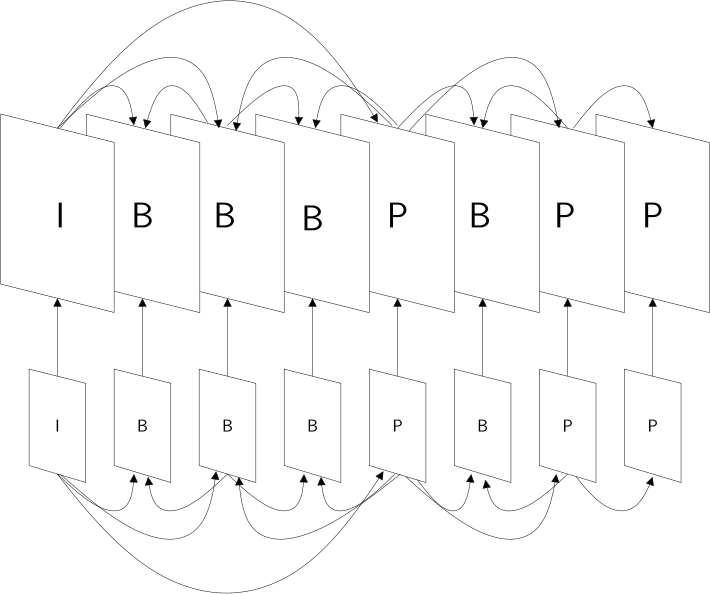
\includegraphics{H264-S-SVC}%{6cm}{600}

\section{Deblocking filtering}
\begin{itemize}
\tightlist
\item
  If any other block-overlaping techniques have not been applied,
  block-based video encoders improve their performance if a deblocking
  filter in used to create the quantized prediction predictions.
\end{itemize}

\includegraphics{350px-Deblock1}%{6cm}{600}

\begin{itemize}
\tightlist
\item
  The low-pass filter is applied only on the block boundaries.
\end{itemize}

\section{Bit-rate allocation}
\begin{itemize}
\item
  VBR: Under a constant quantization level (constant video quality), the
  number of bits that each compressed image needs depends on the image
  content (Variable Bit-Rate). Example:
  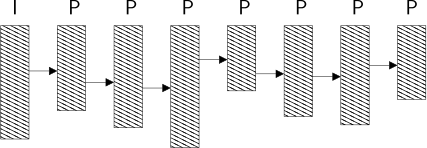
\includegraphics{closed-loop-1_ir}%{6cm}{600}

\item
  CBR: Using a Constant Bit-Rate strategy, all frames need the same
  space. Example:
  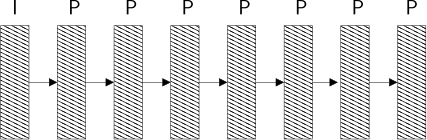
\includegraphics{CBR}%{6cm}{600}
\end{itemize}

\section{Video scalability}
\subsection{Quality scalability}
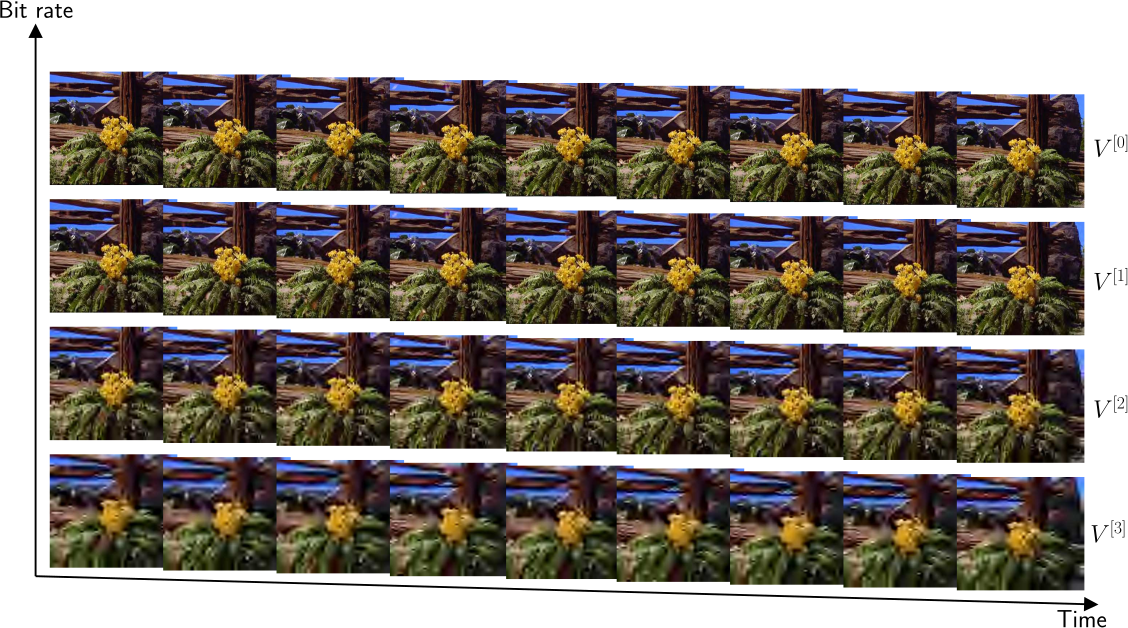
\includegraphics{quality-scalability}%{10cm}{1000}
\begin{itemize}
\item
  Ideal for remote visualization environments.
\item
  By definition, $s^{[0]}:=s$.
\end{itemize}

\subsection{Temporal scalability}
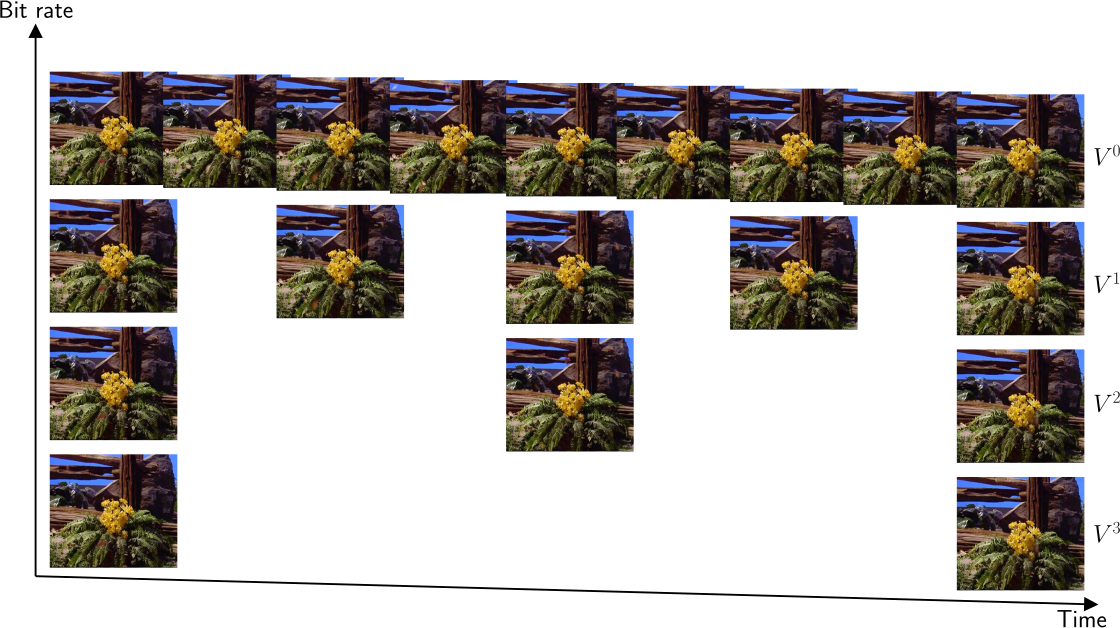
\includegraphics{temporal-scalability}%{10cm}{1000}
\begin{itemize}
\item
  It holds that

  \begin{equation}
    s^{t}=\{s_{2^t i}\}=\{s_{2i}^{t-1}\},
  \end{equation}

  where $t$ denotes the Temporal Resolution Level (TRL).
\item
  Notice that $s:=s^{0}$.
\item
  Useful for fast random access.
\end{itemize}

\subsection{Spatial scalability}
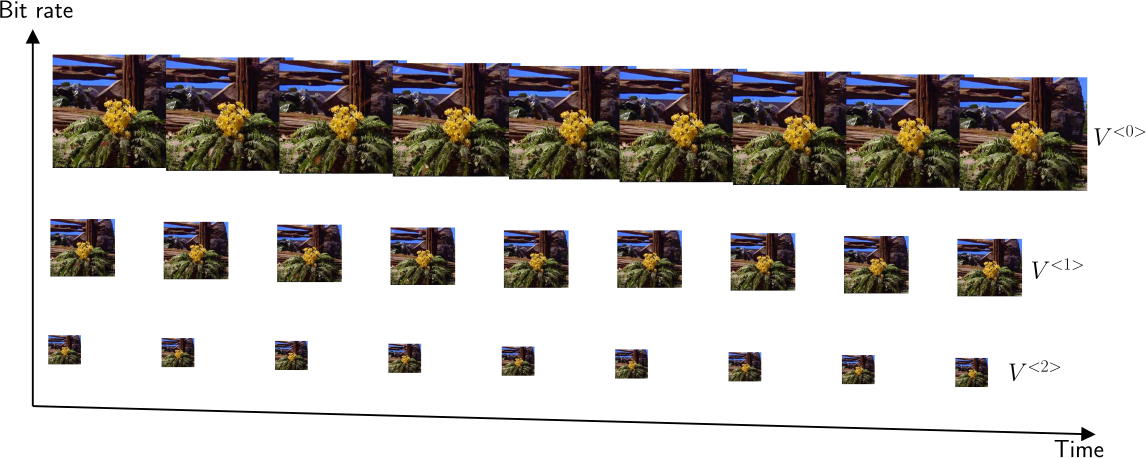
\includegraphics{spatial-scalability}%{10cm}{1000}
\begin{itemize}
\item
  Useful for low-resolution devices.
\item
  By definition, $V_i:=V_i^{<0>}$ and $V_i^{<s>}$ has a
  $\frac{Y}{2^s}\times \frac{X}{2^s}$ resolution, where $X\times Y$
  is the resolution of $V_i$.
\end{itemize}

\bibliography{video-compression}
